	%\addcontentsline{toc}{chapter}{Conclusion générale} 
	\chapter{Conclusion générale}
	\minitoc
	\newpage
	 \label{conclusion-fin}
	\section{Récapitulatif de notre contribution}
	%à faire : rappeler le problème dans le premier paraphe et rappeler les conclusions des expérimentations de chaque chapitre
	
	L'objectif de ce manuscrit était de présenter toutes les méthodes qu'on a implémenté pour tenter de résoudre le problème qu'on a nommé SMEPC (voir sa description détaillée à la section \ref{Le modèle SMEPC}). Le problème est de planifier les recharges d'un véhicule dont on connait la tournée sachant que les quantités d'énergie rechargées devront préalablement être produite par une machine de production. 
	Dans ce manuscrit, on a présenté plusieurs méthodes de résolution du problème SMEPC. On a principalement six chapitres. 
	
	Le \textbf{chapitre} \ref{Etat_art_probleme} fait un état de l'art du problème SMEPC. A notre connaissance, il n'existe aucun article qui traite notre problème mais par contre on a trouvé des articles qui traitent certains aspects de notre problème. On a commencé ce chapitre par l'état de l'art des problèmes de planification de tournées de véhicules qui tiennent compte de l'alimentation des véhicules. On a présenté les problèmes GVRP, PRP, EVPRP, HVRP et RVRP. On poursuivi ce chapitre en présentant ce qu'est un problème de planification de la production. On a conclu ce chapitre en identifiant quelques problématique de synchronisation à savoir la synchronisation discrète et la synchronisation continue.
	
	Le \textbf{chapitre} \ref{Etat_art_methode} fait un état de l'art des méthodes explorées pour résoudre le problème SMEPC. On commence par présenter quelques généralités sur la programmation linéaire en nombres entiers et sur le \textit{Branch-And-Cut}. Puis on poursuit en présentant ce qu'est la programmation dynamique en donnant deux exemples de son utilisation sur deux problèmes connus : le problème du sac à dos et le \textit{Split}. On présente comment les problèmes Stochastiques et cycliques peuvent être traités avec cette technique. On finit ce chapitre en présentant ce qu'est l'apprentissage automatique. On se concentre principalement sur les réseaux de neurones et sur l'API Keras de Tensorflow Keras  qui sert à les implémenter.
	
	Le \textbf{chapitre} \ref{MIP_3_plus} commence par expliquer le problème SMEPC, ensuite on présente sa formulation mathématique notamment ses variables, sa fonction objectif et ses contraintes. Puis, on donne sa formulation linéaire en nombres entiers qu'on nomme $MILP_{SMEPC}$ puis sa relaxation linéaire qu'on nomme $RMILP_{SMEPC}$. On étudie la contribution de plusieurs contraintes nommées $STC$ et $EC$ qui améliorent la relaxation linéaire. On étudie la complexité de notre problème et on finit ce chapitre en présentant les résultats des expérimentations numériques effectuées. La phase expérimentale montre que le modèle $MILP_{SMEPC}$ a du mal à résoudre des instances de \og grandes \fg{} tailles.
	
	Le \textbf{chapitre} \ref{SMEPC_programmation} propose un algorithme de programmation dynamique pour tenter de résoudre le problème SMEPC. On nomme cet algorithme $DPS_{SMEPC}$, on présente l'espace temps, les états, les variables de décisions, les transitions et la mise en œuvre algorithmique de cet algorithme. On propose un schéma d'approximation polynomial. Pour éviter une explosion du nombre d'états, on présente deux types de mécanismes de filtrage : les mécanismes de filtrages exactes (filtrage logique et filtrage par estimation optimiste) et les mécanismes de filtrages heuristiques. On décrit une heuristique rapide nommée $He$ qui calcule une solution de notre problème très rapidement. On finit ce chapitre en présentant les résultats des expérimentations numériques effectuées. 
	
	Il a été constaté que le problème SMEPC peut être divisé en deux sous-problèmes à savoir le problème \textit{Vehicle-Driver} et le problème \textit{Production-Manager}. Le \textbf{chapitre} \ref{Heuristique} se focalise sur un schéma collaboratif nommé \textbf{Pipe-line VD\_PM} qui émule une interaction entre ces deux sous-problèmes. On a commencé ce chapitre en présentant ce qu'est le problème VD et le problème PM. Ensuite, on présente un algorithme de programmation dynamique pour chacun de ces problèmes qu'on nomme $DPS\_VD$ et $DPS\_PM$. Comme pour le $DPS_{SMEPC}$, le problème PM étant le plus difficile, on diminue le nombre d'états produit par le $DPS\_PM$ à l'aide de mécanismes de filtrage. On finit ce chapitre en présentant les résultats des multiples expériences effectuées.
	
	Concernant la programmation dynamique, de toutes les expérimentations effectuées tout au long de ce manuscrit, on conclut que le filtrage heuristique est très efficace pour filtrer les états. De plus, le filtrage par estimation optimiste est le filtrage exacte le plus efficace. 
	
	Dans le \textbf{chapitre} \ref{neurones}, on tente de construire un estimateur rapide du coût de la solution optimale d'une instance. Cet estimateur est construit à l'aide de réseaux de neurones. On commence par construire deux réseaux \og simples\fg{} qu'on nomme SIMPLE\_TYPE et SIMPLE\_PERIODE. Ensuite on construit un réseau MIXTE\_COUT et MIXTE\_TEMPS qui essayent d'épouser les caractéristiques du problème. %Ces quatre réseaux prédissent le coût de production car comme on l'a constaté c'est ce sous-problème le plus difficile des deux.
	 Les instances étant utilisées comme entrées de nos réseaux, cela a pour conséquence une importante augmentation du nombre de neurones. Pour résoudre ce problème on va construire les réseaux INDIC\_COUT et INDIC\_TEMPS dont les entrées seront des indicateurs qui sont une agrégation des instances. La phase expérimentale nous montre que les réseaux INDIC\_COUT et INDIC\_TEMPS sont les plus performants.
	
	
	
\section{Perspectives}
	Nous constatons que notre problème peut être étendu, notamment :
	\begin{itemize}[label=$\square$]
			\item en supposant que l'optimisation de la tournée fait partie du processus de prise de décision ;
		\item en supposant que les valeurs de rendement $R_i$ sont gérés comme des quantités non déterministes.
	\item en supposant que le véhicule est alimenté avec plusieurs types d'énergies ;
	\item en supposant qu'on a plusieurs véhicules pour effectuer les différentes tâches ;
 
	\end{itemize}
	
	
	%\subsection{Extensions du problème SMEPC}
	\label{extensions_SMEPC}
	On pourrait concevoir un modèle qui optimise la tournée du véhicule en utilisant le modèle basé sur les techniques d'apprentissage du dernier chapitre. Plus concrètement, On peut évaluer la qualité d'une tournée avec l'algorithme Pipe-line VD\_PM dans lequel on va remplacer le module DPS\_PM par le réseau de neurones basé sur les indicateurs. Avant cela, on va entrainer le réseau de neurones qui nous permettra de prédire le coût d'une solution de SMEPC. Nous supposons également que nous disposons d'un opérateur de recherche locale qui modifie la tournée en effectuant une séquence d'opérations de suppression, suivie d'une séquence d'opérations de réinsertion de stations.
	
	On pourrait réfléchir comment ajouter de la robustesse à nos algorithmes pour que même si les rendements sont inférieurs aux prévisions que cela n'entraine pas que les stratégies de production et de recharge soient non réalisables. Nous revenons donc ici au problème global SMEPC, et considérons que les rendements de production $R_i$ doivent être gérés comme des quantités non déterministes. Le cadre standard de programmation dynamique stochastique, basé sur des hypothèses markoviennes (Voir section \ref{markov}), ne peut être utilisé ici, puisqu'il existe clairement des corrélations entre les $R_i$. Au lieu d'utiliser donc la programmation dynamique stochastique,on peut s'appuyer sur la notion de \textbf{scénario}.  Un scénario est une hypothèse de comportement global de l'évolution du $R_i$, qui peut également être considéré comme une hypothèse sur la façon dont le temps évolue au cours des périodes $0, \dots, N-1$.
	
	Le problème \textbf{SMEPC} peut être étendu en modifiant ses caractéristiques. Si on décide que le véhicule fonctionne avec deux types d'énergies, par exemple l'hydrogène et l'électricité. Ceci signifie que le véhicule contient une pile à hydrogène pour conserver l'hydrogène et une batterie pour stocker l'électricité. L'une des difficultés ici serait de calculer quelle proportion d'hydrogène et d'électricité le véhicule devrait dépenser pour se déplacer d'une station à l'autre. De plus, il faudrait décider quelles proportions d'hydrogène et d'électricité seront rechargée lorsque le véhicule ira se recharger.
	
	Si on décide qu'il y a plusieurs véhicules (au lieu d'un seul) pour effectuer les tâches de logistique interne, on a plusieurs difficultés : l'une est d'empêcher les collisions entre les véhicules en faisant en sorte qu'ils ne se croisent jamais sur la même route ou à un carrefour. Une autre difficulté est d'attribuer des tâches de façon optimale à chaque véhicule. Aussi, on doit gérer une file d'attente au niveau de la micro-usine car les véhicules peuvent s'y retrouver à plusieurs. Une autre difficulté est d'optimiser les tournées des véhicules.
	
	
	 Le paragraphe suivant sera consacré à la présentation plus ou moins exhaustive de façon précise des extensions possibles du problème \textbf{SMEPC}. 
	Parmi les variants du problème \textbf{SMEPC} avec tournée fixée, on peut citer :
	
	\begin{enumerate}%[label=$\square$]
		\item On suppose que la quantité d'hydrogène rechargée par le véhicule est la même à chaque recharge, la recharge dure une période. La quantité d'hydrogène produite est variable (La micro-usine produit à chaque pas de temps une quantité d'hydrogène comprise entre 1 et un seuil max à fixer.). Le véhicule n'attend pas au niveau de la micro-usine, il se recharge immédiatement car il est prioritaire ;
		\item On suppose que la quantité d'hydrogène rechargée par le véhicule est la même à chaque recharge, la recharge dure une période. La quantité d'hydrogène produite est fixe (La micro-usine produit à chaque pas de temps une quantité d'hydrogène connue.). Le véhicule n'attend pas au niveau de la micro-usine, il se recharge immédiatement car il est prioritaire ;
		\item On suppose que la quantité d'hydrogène rechargée par le véhicule est la même à chaque recharge, la recharge se fait en $\delta$ périodes de temps. La quantité d'hydrogène produite est fixe et on n'a pas de temps d'attente  ;
		\item Le véhicule fait le plein de son réservoir d'hydrogène à chaque recharge, la recharge se fait en $\delta$ périodes de temps, la quantité d'hydrogène produite est fixe et on n'a pas de temps d'attente ;
		\item Le véhicule fait le plein de son réservoir d'hydrogène à chaque recharge, la recharge dure une période, la quantité d'hydrogène produite est fixe et le véhicule peut attendre à la micro-usine (par exemple il peut attendre que la micro-usine produise la quantité dont il a besoin). Ce dernier cas est le problème SMEPC.
	\end{enumerate}
	
	Le tableau (\ref{syn_variant}) synthétise les variants du problème \textbf{SMEPC} présenté ci-dessus.
	
	\begin{table}[H]
		\begin{center}
			
			\begin{tabular}{|l|l|l|l|l|l|l|}
				\hline
				%\multicolumn{3}{|c|}{Synthèse de quelques variants} \\
				%\hline
				Caractéristiques & Possibilités &  &&&&SMEPC\\ \hline
				Quantité rechargée & fixe & 1&2&3&& \\
				& Variable &  &&&4&5\\\hline
				Durée de la recharge &  $\delta$ périodes &  &&3&4&\\
				& 1 période & 1&2&&&5\\\hline
				Quantité produite &fixe &  &2&3&4&5\\%$\boxtimes$
				& variable &1  &&&&\\
				\hline
				Attente avant recharge & oui & &&&&5\\
				& non & 1&2&3&4&\\
				\hline
			\end{tabular}
		\end{center}
		\caption[Synthèse de quelques variants du problème SMEPC ]{Synthèse de quelques variants du problème \textbf{SMEPC}.\label{syn_variant} }
	\end{table}
	
	%De nombreuses questions restent à résoudre notamment étendre notre approche à plusieurs véhicules ; adapter les algorithmes à l'optimisation de la tournée. Les section suivantes sont consacrées à la présentation brève de deux perspectives notamment l'inclusion de la tournée du véhicule dans la décision et à la question de la robustesse à travers la gestion des incertitudes.
	
	
	
\poubelle{
	%\section{Perspectives}
	\section{Perspective 1 : Le parcours du véhicule comme élément de la décision}
	\label{design_tour}
	\subsection{Algorithme d'optimisation de la tournée}
	
	Dans cette section, notre but est de présenter une perspective de notre problème. C'est le problème qui consiste à optimiser la tournée $\Gamma$ du véhicule. On présente donc l'algorithme qui nous servira à optimiser la tournée du véhicule. On veut dans cette section concevoir un modèle qui optimise la tournée du véhicule en utilisant le modèle basé sur les techniques d'apprentissage du chapitre précédent. Plus concrètement, On va évaluer la qualité d'une tournée avec l'algorithme Pipe-line VD\_PM auquel on va remplacer le module DPS-PM par le réseau de neurones basé sur les indicateurs du chapitre précédent. Avant cela, on va entrainer un réseau de neurones qui nous permettra de prédire le coût d'une solution de SMEPC.
	%L'objectif de ce chapitre était de présenter un réseau de neurones qui nous servirait à ajouter l'optimisation de la tournée du véhicule au problème SMEPC. Ce modèle est utilisé pour optimiser la tournée du véhicule.
	 Optimiser ici signifie que nous voulons que $\Gamma$ soit tel que la valeur du coût global $W$ obtenue par l'application de l'algorithme du pipeline (corresponds aux algorithme (\ref{DPS-VEHICULE}), (\ref{Primary-Refueling }) et (\ref{Reduced-Refueling})) \textbf{DPS\_VD} à $\Gamma$ soit la plus petite possible.  
	Nous supposons donc ici que nous disposons d'une telle tournée $\Gamma = \{Depot = 0, 1, \dots, j, \dots, M, Depot=M+1\}$, et que nous avons appliqué la procédure de programmation dynamique \textbf{DPS\_VD} à $\Gamma$. Cela signifie que nous disposons d'une stratégie de recharge réduite $\sum$ caractérisée par $Q$, $m_q$, $M_q$.
	
	Nous supposons également que nous disposons d'un opérateur de recherche locale (Suppression\_Insertion) $R\_I(\Gamma, J)$, qui modifie $\Gamma$ en considérant un certain sous-ensemble $J$ de l'ensemble des stations $1, \dots, M$, en effectuant une séquence d'opérations de suppression, suivie d'une séquence d'opérations de réinsertion de stations. Il s'avère que la question que nous allons discuter ici porte sur la manière dont nous pouvons contrôler l'application de cet opérateur, en tenant compte des informations contenues dans $\sum$ . 
	Une façon de procéder pour réaliser l'optimisation de $\sum$ est d'utiliser une des formules d'approximation $A(\sum)$ (indicateurs ou réseau de neurones) que nous avons étudier précédemment, et de faire comme si notre but était de minimiser $A(\sum)$. On peut par exemple effectuer une boucle de descente comme le montre l'algorithme (\ref{Tour}). Une autre façon de procéder pour réaliser l'optimisation de $\Gamma$ est de ne s'intéresser qu'à la valeur $V^\lambda= \alpha.T + \lambda .E$ calculée par DPS\_VD(), où $E$ est la quantité d'énergie requise par le véhicule pour réaliser la tournée $\Gamma$ , $T$ est la durée de $\Gamma$ , et $\lambda$ est le coefficient de prix unitaire de l'énergie que nous utilisons lors de l'application de DPS\_VD(). Cela signifie que notre objectif intermédiaire (avant de revenir à la vraie valeur de W) est de minimiser $V^\lambda(\Gamma)$.
	
	
	\begin{algorithm}
		\caption{Tour}
		\label{Tour}
		\begin{algorithmic}[1]
			\REQUIRE $Seuil$
			\ENSURE $\Gamma$
			\hline
			\vspace{0.5cm}
			
			\INITIALISATION
			\STATE $NotStop$ ;
			\STATE Initialiser $\Gamma$ ;
			\STATE $\sum \leftarrow DPS\_VD(\Gamma)$ ;
			\STATE $W\_Aux \leftarrow A(\sum)$ ;
			
			\vspace{0.3cm}
			
			\BOUCLEPRINCIPAL
			\WHILE{$NotStop$}
			\STATE $Counter \leftarrow 0 $ ;
			\STATE $NotStop1$ ;
			\WHILE{$Counter \leq Seuil \land NotStop1$}
			\STATE Générer un sous-ensemble de station $J$ ; \label{generate}
			\STATE $\Gamma\_Aux \leftarrow R\_I(\Gamma,J)$ ; \label{RI}
			\STATE $\sum\_Aux \leftarrow$ DPS\_VD($\Gamma\_Aux$) ;
			\STATE $W\_Aux \leftarrow A(\sum\_Aux)$ ;
			\IF{$W\_Aux < W$}
			\STATE $ \Gamma \leftarrow \Gamma\_Aux$ ; $\sum \leftarrow \sum\_Aux$ ; $ W \leftarrow W\_Aux$ ; $Stop1$ ;
			\ELSE
			\STATE $Counter \leftarrow Counter +1$ ;
			\IF{$Counter > Seuil$}
			\STATE $Stop$ ;
			\ENDIF
			\ENDIF
			\ENDWHILE
			\ENDWHILE
		\end{algorithmic}
	\end{algorithm}
	
	
	Nous pouvons facilement randomiser (schéma GRASP) l'algorithme (\ref{Tour}) en rendant le processus d'initialisation déterministe, et en plaçant l'algorithme (\ref{Tour}) dans un cadre multi-départ. Dans tous les cas, nous calculerons une ou plusieurs paires $(\Gamma,\sum )$, qui seront entièrement évaluées par l'application de la procédure \textbf{DPS\_PM}. Le schéma GRASP consiste à génèrer plusieurs solutions dans l'espace des solutions possibles d'un problème, à l'aide par exemple d'un algorithme glouton randomisé puis, à améliorer chaque solution obtenue à l'aide par exemple d'une recherche locale et enfin à sélectionner la meilleure solution parmi ces solutions améliorées. Cela s'effectue en deux principales phases : la phase de
	construction d'une solution et la phase d'amélioration de celle-ci. Ce processus est répété
	tant qu'une certaine condition préalablement fixée n'est pas satisfaite. Cette condition
	peut par exemple être un certain nombre d'itérations à effectuer.
	
	Dans cette perspective, les instructions clés sont l'instruction (\ref{generate}) et l'instruction (\ref{RI}) qui commande la réinsertion du sous-ensemble de stations $J$ dans $\Gamma$. Les procédures exécutant ces instructions sont décrites à la section suivante.
	\subsection{Opérateurs de suppression et d'insertion}
	
	Lorsque nous exécutons les instructions (\ref{generate}) et (\ref{RI}) de l'algorithme (\ref{Tour}), nous nous basons sur la tournée actuelle $\Gamma$ et de la stratégie de recharge $\sum$. Cette stratégie de recharge permet de diviser $\Gamma$ en une séquence de $Q+1$ sous-tours qu'on nomme $\Gamma_0, \dots, \Gamma_Q$ (où $Q$ est le nombre d'opérations de recharge) de la façon suivante :
	\begin{itemize}[label=$\square$]
		\item $j_1, \dots, j_Q$ sont les stations de $\Gamma$ juste après lesquelles le véhicule fait un détour c'est-à-dire qu'il va à la micro-usine se recharger. Et les stations $j^*_1, \dots, j^*_Q$ sont leurs successeurs dans $\Gamma$ ;
		\item Nous supposons que les stations sont étiquetées de telle sorte que $\Gamma = \{Depot=0, 1, \dots, M, M+1=0=Depot \}$ ;
		\item $\Gamma_0 = \{Depot=0, 1, \dots, j_1, Depot\}$ ;
		%!!!!!!!!!!!!!!!question Al: peut-on se recharger après le dépôt avec cette formule ?
		\item $\Gamma_q = \{Depot=0, j^*_q, \dots, j_{q+1}, Depot\}$, pour $q=1, \dots, Q-1$ ;
		\item $\Gamma_Q=\{Depot=0, j^*_Q, \dots, M, Depot\}$. %!!!!!!!!!!!!!!!question Al: peut-on se recharger après la station M avec cette formule ?
		
	\end{itemize}
	
	De plus, nous désignons par :
	
	\begin{itemize}[label=$\square$]
		\item $L$ la longueur (au sens temps) de $\Gamma$ (sans ajouter les détours);
		\item $\Delta$ la longueur (au sens énergie) de $\Gamma$ (sans ajouter les détours) ;
		\item $T$ et $E$ comme ci-dessus, sont respectivement la longueur au sens temps et la longueur au sens énergie de la tournée $Gamma$ complété par les détours induit par les opérations de recharge. 
	\end{itemize}
	
	Nous faisons comme si nous avons affaire au problème VRP qu'on nomme \textbf{VRP\_ET} suivant :
	
	\{Calculons une collection de tournées $\gamma_0, \dots, \gamma_K$, telle que :
	\begin{itemize}[label=$\square$]
		\item La valeur $\sum_k (\alpha.L_E(\gamma_k) + \lambda.L_T(\gamma_k))$ est la plus petite possible. Ici, $L_E(\gamma_k)$ est la longueur de $\gamma_k$ au sens énergie, et $L_T(\gamma_k)$ est la longueur de $\gamma_k$ au sens temps, $k$ faisant partie du problème ; 
		\item Pour tout $k$ : $L_E(\gamma_k) \leq C^{Veh}$ car le véhicule ne peut se recharger qu'au maximum  d'une quantité de carburant $C^{Veh}$ ;
		\item $L_E(\gamma_0) \leq E_0$ car le véhicule commence sa tournée avec une quantité de carburant $E_0$ ; 
		%!!!!!!!!!!!!!!!question Al: peut-on se recharger après le dépôt avec cette formule ?
		\item $L_E(\gamma_K) \leq C^{Veh} -E_0$ car le véhicule doit finir sa tournée avec une quantité de carburant au moins égale à $E_0$.\}
		%!!!!!!!!!!!!!!!question Al: peut-on se recharger après la station M avec cette formule ?
		
	\end{itemize}
	\subsubsection{Opérateur de suppression}
	Les fonctions $First(\gamma_k)$ et $Last(\gamma_k)$ permettent d'obtenir respectivement la première et la dernière station (différente du dépôt) de $\gamma_k$. Les fonctions $Time(j,j')$ et $Energy(j,j')$ permettent d'obtenir respectivement la longueur au sens temps et la longueur au sens énergie entre la station $j$ et la station $j'$.
	
	Selon ce qui vient d'être dit aux sections précédentes, nous voyons que nous avons affaire à $K =Q$ et à une solution actuelle de \textbf{VRP\_ET} $\gamma=\{\Gamma_0=\gamma_0, \dots, \gamma_K=\Gamma_Q\}$. Afin d'effectuer cette étape de suppression, nous avons d'abord besoin de choisir le nombre $C\_j$ de stations qui vont être supprimées de la tournée actuelle $\gamma_k, k=0, \dots, K$. Une fois que cela a été fait, nous disons qu'une station $j$ sera candidate à la suppression si :
	\begin{itemize}[label=$\square$]
		\item En enlevant $j\in \gamma_k$, $j\neq Depot$,  on a une diminution significative de $L_E(\gamma_k)$ ou de $L_T(\gamma_k)$.
		% On peut par exemple choisir d'enlever la station qui entraine la diminution la plus élevée ;
		\item $j = First(\gamma_k)$, $j\_Ant = Last(\gamma_{k-1})$ :
		
		la longueur du détour en temps
		$Time(j\_Ant, Depot) + Time(Depot, j) - Time(j\_Ant, j)$
		est élevée
		
		ou la longueur du détour en énergie 
		$Energy(j\_Ant, Depot) + Energy(Depot, j) - Energy(j\_Ant, j)$ est élevée ;
		\item $j = Last(\gamma_k)$, $j\_Succ = First(\gamma_{k+1})$ :
		
		la longueur du détour en temps $Time(j, Depot) + Time(Depot, j\_Succ) - Time(j, j\_Succ)$ est élevée
		
		ou la longueur du détour en énergie $Energy(j, Depot) + Energy(Depot, j\_Succ) - Energy(j, j\_Succ) $ est élevée ; 
		%!!!!!!!!!!!!Cest qui une diminution significative
		%!!!! on peut par exemple choisir d'enlever la station qui entraine la diminution la plus élevée 
		%Pour l'implémentation on a retirer les stations dont beta*energie +alpha*temps est supérieurs à la moyenne des beta*energie+alpha*temps de toutes les stations. energie et temps sont remplacés par les formules ci-dessus
	\end{itemize}
	
	%Pour savoir que la longueur d'un détour est élevé on peut par exemple décider que c'est lorsque cette longueur est supérieure à la moyenne des longueurs des détours de toutes les stations. On peut donc décider de supprimer les $C\_J$ stations qui respectent cette dernière condition. 
	On effectue l'étape de suppression avec l'algorithme (\ref{Supp}).
	\begin{algorithm}
		\caption{Suppression}
		\label{Supp}
		\begin{algorithmic}[1]
			\REQUIRE $\gamma$, $C\_J$
			\ENSURE $\gamma$
			\hline
			\vspace{0.5cm}
			
			\INITIALISATION
			\STATE Calculer un ensemble $J\_Removal$ de stations candidates à la suppression ;
			
			\vspace{0.3cm}
			
			\BOUCLEPRINCIPAL
			\FOR{$c = 1$ \TO $C\_J$}
			\STATE Sélectionner de façon aléatoire $j$ dans $J\_Removal$ et supprimer cela de $\gamma$ ;
			\ENDFOR
		\end{algorithmic}
	\end{algorithm}
	
	\subsubsection{Opérateur d'insertion}
	On effectue l'étape d'insertion avec l'algorithme (\ref{Insert}).
	\begin{algorithm}
		\caption{Insertion}
		\label{Insert}
		\begin{algorithmic}[1]
			\REQUIRE $\gamma_0, \dots, \gamma_K$
			\ENSURE 
			\hline
			\vspace{0.5cm}
			
			\INITIALISATION
			\STATE Concaténer les tournées $\gamma_0, \dots, \gamma_K$  tels qu'elles sont après l'étape de suppression, en une tournée unique $\Pi$ sans aucun détour ;
			\STATE Appliquer DPS\_VD($\lambda$) à $\Pi$ et une nouvelle collection de tournées $\gamma^*=\{\gamma^*_0, \dots, \gamma^*_K^*\}$
			\STATE $J \leftarrow$ \{les stations j à reinsérer\}%C'est à cette étape que le code C++ s'arrête
			
			\vspace{0.3cm}
			
			\BOUCLEPRINCIPAL
			\WHILE{$J \neq Nil$}
			\STATE Sélectionner de façon aléatoire $j$ dans $J$ et supprimer $j$ de $J$
			\STATE Insérer $j$ dans $\gamma^*$ de telle sorte que les contraintes \textbf{VRP\_ET} restent satisfaites et que l'objectif $\sum_k (\alpha.L_E(\gamma_k) + \lambda.L_T(\gamma_k))$ reste le plus petite possible (meilleur principe d'insertion) /*remarquez que cela peut faire augmenter $K^*$, avec la création d'une tournée supplémentaire $\{Depot, j, Depot\}$ ; Dans ce cas, cette tournée supplémentaire est insérée aléatoirement n'importe où dans la collection $\gamma^*$*/ ;
			\ENDWHILE
		\end{algorithmic}
	\end{algorithm}
	
	
	\subsubsection{Détails des instructions (\ref{generate}) et (\ref{RI}) de l'algorithme (\ref{Tour})}
	En fait, nous voyons que nous pouvons remplacer les instructions (\ref{generate}) et (\ref{RI}) de l'algorithme (\ref{Tour}) par l'algorithme (\ref{RII}).
	\begin{algorithm}
		\caption{R\_I}
		\label{RII}
		\begin{algorithmic}[1]
			\REQUIRE $\{\Gamma_0, \dots, \Gamma_Q\}$%$\Gamma$, $J$
			\ENSURE $\Gamma$
			\hline
			\vspace{0.5cm}
			
			\INITIALISATION
			%\STATE $K\leftarrow Q$ ;
			\STATE  $\gamma $ $\leftarrow \{ \Gamma_0, \dots, \Gamma_Q\}$ ;/*$\gamma $ est la solution actuelle de \textbf{VRP\_ET}*/
			
			\vspace{0.3cm}
			
			\BOUCLEPRINCIPAL
			\WHILE{ $\gamma$ n'est pas un optimum local de \textbf{VRP\_ET}}
			\STATE Appliquer les opérateurs d'insertion et de suppression à  $\gamma$ ;
			\ENDWHILE
			\STATE Reconstruire $\Gamma$ de $\gamma$ ;
		\end{algorithmic}
	\end{algorithm}
	
\section{Perspective 2 : La gestion des incertitudes sur les rendements }
Le but de cette section est d'expliquer comment ajouter de la robustesse à nos algorithmes pour que même si les rendements sont inférieurs aux prévisions que cela n'entraine pas que les stratégies de production et de recharge soient infaisables.
\subsection{Définition de scénario}

Nous revenons donc ici au problème global SMEPC, et considérons que les rendements de production $R_i$ doivent être gérés comme des quantités non déterministes. Le cadre standard de programmation dynamique stochastique, basé sur des hypothèses markoviennes (Voir section \ref{markov}), ne peut être utilisé ici, puisqu'il existe clairement des corrélations entre les $R_i$. Au lieu d'utiliser donc la programmation dynamique stochastique, nous nous appuyons sur la notion de \textbf{scénario}. 

Un scénario est une hypothèse de comportement global de l'évolution du $R_i$, qui peut également être considéré comme une hypothèse sur la façon dont le climat évolue pendant les périodes $0, \dots, N-1$. Il peut être interprété de 2 façons :

\begin{itemize}[label=$\square$]	
\item \textbf{Évolution Faible} : un scénario est une séquence de valeurs $R_i$, $i = 0, \dots, N-1$ ;
\item \textbf{Évolution Forte} : un scénario est un mot $\sigma$, écrit avec un alphabet donné $A$ , et à chaque symbole $s$ de $\sigma$ , correspond une certaine valeur de rendement de production moyen $R(s,\sigma )$ et une certaine fenêtre temporelle $\{Inf(s, \sigma), \dots, Sup(s,\sigma )\}$ dans $\{0, \dots, N-1\}$.
\end{itemize}

Pour des raisons de simplicité, nous nous limiterons ici à la notion de faible scénario.

Nous traitons l'incertitude en considérant que nous disposons d'une collection  $\sum$ (de petite taille) de scénarios $\sigma$, qui définit un arbre de scénarios : 

\begin{itemize}[label=$\square$]	
\item Un scénario partiel $\tau$ est la restriction d'un certain scénario $s$ aux périodes $0, \dots, i_0-1$ où $i_0$ est une période donnée ; Le scénario vide ($i_0 = 0$) est noté $Nil$ ;
\item Pour tout $i_0$, et tout scénario partiel $\tau$, nous désignons par $\sum(i_0,\tau )$ le sous-ensemble $\sum$ de scénarios $\sigma$ dont la restriction jusqu'à $i_0-1$ est $\tau$ .
\item Lorsque, à une certaine période $i_0$, un scénario partiel $\tau$ donne lieu à différents scénarios partiels $\tau_1, \dots, \tau_H$, nous considérons que ce processus de découpage est stochastique, et effectué selon une distribution de probabilité $Q(i_0,\tau) = (Q(i_0,\tau_h), h = 1, \dots, H)$. Ces distributions sont indépendantes. 
\end{itemize}

 La figure (\ref{scenarios}) présente un exemple d'arbre de scénarios avec 3 scénarios. Ces 3 scénarios se divisent une première fois à la période $i_0 = 8$, selon la distribution de probabilité $(0.5, 0.5)$, en un scénario global $\sigma_3$ et un scénario partiel $\tau$, qui à son tour se divise à la période 14 en scénarios globaux $\sigma_1$ et $\sigma_2$, selon la distribution $(0.7, 0.3)$. 
 
 \begin{figure}
 	\centerline{
 		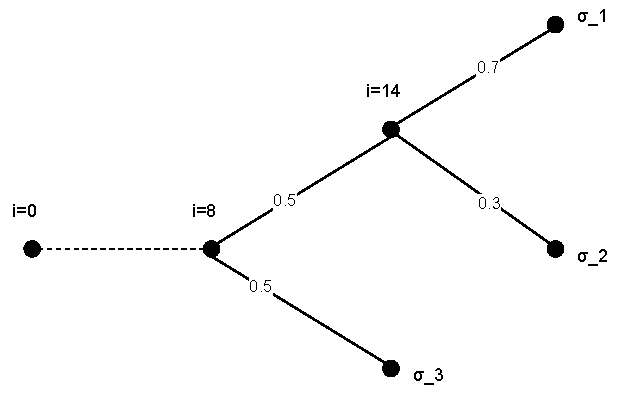
\includegraphics[width=9cm]{images_these/scenarios.pdf}}
 	\caption{Exemple d'arbre de scénarios}\label{scenarios}
 \end{figure}
 \subsection{Adaptation de SMEPC aux scénarios}
 
 Puisque nous avons conçu un scénario déterministe selon une stratégie forward, ce qui nous a permis de mettre en œuvre des dispositifs de filtrage backward, nous aimerions faire de même en pensant au cas non déterministe.  Cependant, nous sommes confrontés à plusieurs difficultés :
 
 \begin{itemize}[label=$\square$]	
 	\item Puisqu'un état à une certaine période $i_0$ impliquera une composante du scénario, nous devons nous attendre à un plus grand nombre d'états que dans le cas déterministe ;
 \item Dans le cas déterministe, nous recherchons une séquence de décision qui va induire une trajectoire. Dans le cas non déterministe, nous devons réfléchir à une stratégie ;
 \item L'évaluation d'une telle stratégie doit prendre en compte à la fois un risque d'échec (nous ne pouvons pas fournir assez de carburant au véhicule), et la valeur du coût attendu induit en cas de succès. 
 \item  Les dispositifs de filtrage dans le cas déterministe étaient basés sur l'anticipation qu'aucune trajectoire réalisable ou de bonne qualité ne pouvait prolonger un certain état actuel. Dans le cas non déterministe, les choses sont plus compliquées, car aucune attente de faisabilité ou de qualité n'est susceptible d'être pondérée par une certaine distribution de probabilité.  
\end{itemize}

 Ainsi, nous nous limitons d'abord au sous-problème de la production qui apparaît dans le schéma de décomposition Pipe-Line. Il est clair que l'incertitude est liée ici au rendement de production $R_i$, $i = 0,\dots, N-1$. Une stratégie de recharge des véhicules peut être calculée sans tenir compte de cette incertitude ce qui nous permet d'adapter plus facilement notre algorithme au cas non déterministe.  
 
 Nous définissons l'objet décisionnel que nous recherchons comme une stratégie $S$ : cela signifie que, pour toute période $i = 0, \dots, N-1$, si nous sommes dans l'état $E$ sous le scénario actuel $\sigma$, nous voulons savoir quelle décision $d = S(i, E, \sigma)$ doit être prise. Une telle stratégie $S$ transformera l'arbre des scénarios en un arbre des trajectoires.  Certaines trajectoires vont donner une certaine valeur de coût $W(\gamma)$ et les autres vont correspondre à un échec. Ainsi, prise dans son ensemble, la stratégie $S$ va produire 2 quantités :
 
  \begin{itemize}[label=$\square$]		
 \item Une valeur attendue $W(S)$ de la valeur $W(\gamma)$ prise pour toutes les trajectoires $\gamma$ qui n'induisent pas un résultat d'échec : cette valeur attendue est conditionnée par le fait que $\gamma$ n'est pas une trajectoire d'échec ;
 
 \item Une valeur de risque d'échec $R\_Fail(S)$, qui est la probabilité que la trajectoire$\gamma$ résultante soit une trajectoire d'échec.
\end{itemize}
Notre problème devient donc bi-objectif : nous voulons minimiser simultanément $W$ et $R\_Fail$.  Mais une telle formulation bi-objective est à la fois ambiguë et difficile à gérer. La levée de l'ambiguïté se fera en imposant un seuil $Risk\_Max$ à $R\_Fail$ puis en minimisant $W$.  

Donc notre problème devient : calculer une stratégie $S$ telle que $R\_Fail(S) \leq  Risk\_Max$ et $Min = W(S)$.

En fait, il arrivera, exactement comme dans le cas déterministe, que notre stratégie ne soit explicitement définie que pour certains 3-uplets $(i, E, \sigma)$ qui ont été générés au cours d'un processus DPS. Si l'état actuel réel $E$ ne correspond pas à cette condition, nous travaillerons par interpolation et appliquerons à $(i, E, \sigma)$ une décision $d = S(i, E^*, \sigma)$, où $E^*$ est proche de $E$ dans un certain sens et tel que $S(i, E^*,\sigma )$ a été explicitement calculé par notre algorithme DPS. 

Enfin, nous posons une hypothèse qui nous permettra de restreindre le risque de défaillance aux cas où le $R_i$ devient trop faible pour permettre de produire la quantité d'énergie requise. Cette hypothèse est la suivante : si, à une période $i$, nous produisons une quantité d'énergie $R_i$ supérieure à $C^{Tank} - V^{Tank}$, alors nous supposons qu'il est possible de se débarrasser de la quantité excédentaire et d'éviter ainsi une configuration d'échec. 
Cette hypothèse écarte le risque de défaillance qui pourrait découler d'une surproduction et d'un manque de capacité de stockage.   
}
%\makeglossaries
%\section{Perspective 3 : Étendre le problème à plusieurs véhicules}	